\chapter{Perancangan}
\label{chap:perancangan}

Bab ini menjelaskan mengenai perancangan yang disusun dari analisis yang dilakukan pada bab 3. Perancangan yang dilakukan mencakupi diagram kelas rinci, diagram \textit{sequence}, serta penjelasan mengenai hasil analisis yang tidak mungkin diimplementasikan dan cara lain yang dilakukan untuk mendapatkan hasil yang serupa.



\section{Perancangan Kelas}
\label{sec:perancangan_kelas}

Gambar \ref{fig:DetailedClassDiagram} menjelaskan mengenai kelas-kelas dalam perangkat lunak yang dibuat. Beberapa kelas utama yang perlu dijelaskan antara lain:

\par{\textbf{MainPage} : Kelas ini merupakan kelas yang berperan sebagai tampilan utama aplikasi. Atribut-atribut yang dimiliki oleh kelas ini adalah:
    \begin{itemize}
        \item{cpd\\Atribut untuk menyimpan \textit{instance} CaptivePortalDetector.}
        \item{timeoutTimer\\Atribut untuk menyimpan timer yang digunakan untuk menghitung \textit{connection timeout}.}
        \item{loaded\\Atribut untuk menyimpan status \textit{loading} suatu halaman.}
    \end{itemize}
    Metode-metode yang dimiliki oleh kelas ini adalah:
    \begin{itemize}
        \item{setup\\Metode ini digunakan untuk melakukan \textit{setup} awal saat aplikasi dieksekusi.}
        \item{MainWebView\_LoadCompleted\\Metode ini dipanggil saat WebView selesai melakukan loading halaman.}
        \item{MainWebView\_NavigationStarting\\Metode ini dipanggil saat WebView baru akan memulai navigasi ke halaman baru.}
        \item{MainWebView\_NewWindowRequested\\Metode ini dipanggil saat WebView melakukan \textit{request} untuk membuka window baru.}
        \item{MainWebView\_NavigationCompleted\\Metode ini dipanggil saat WebView selesai melakukan navigasi ke halaman baru, namun belum selesai melakukan loading halaman tersebut.}
    \end{itemize}
}

\begin{figure}[!htb]
    \centering
    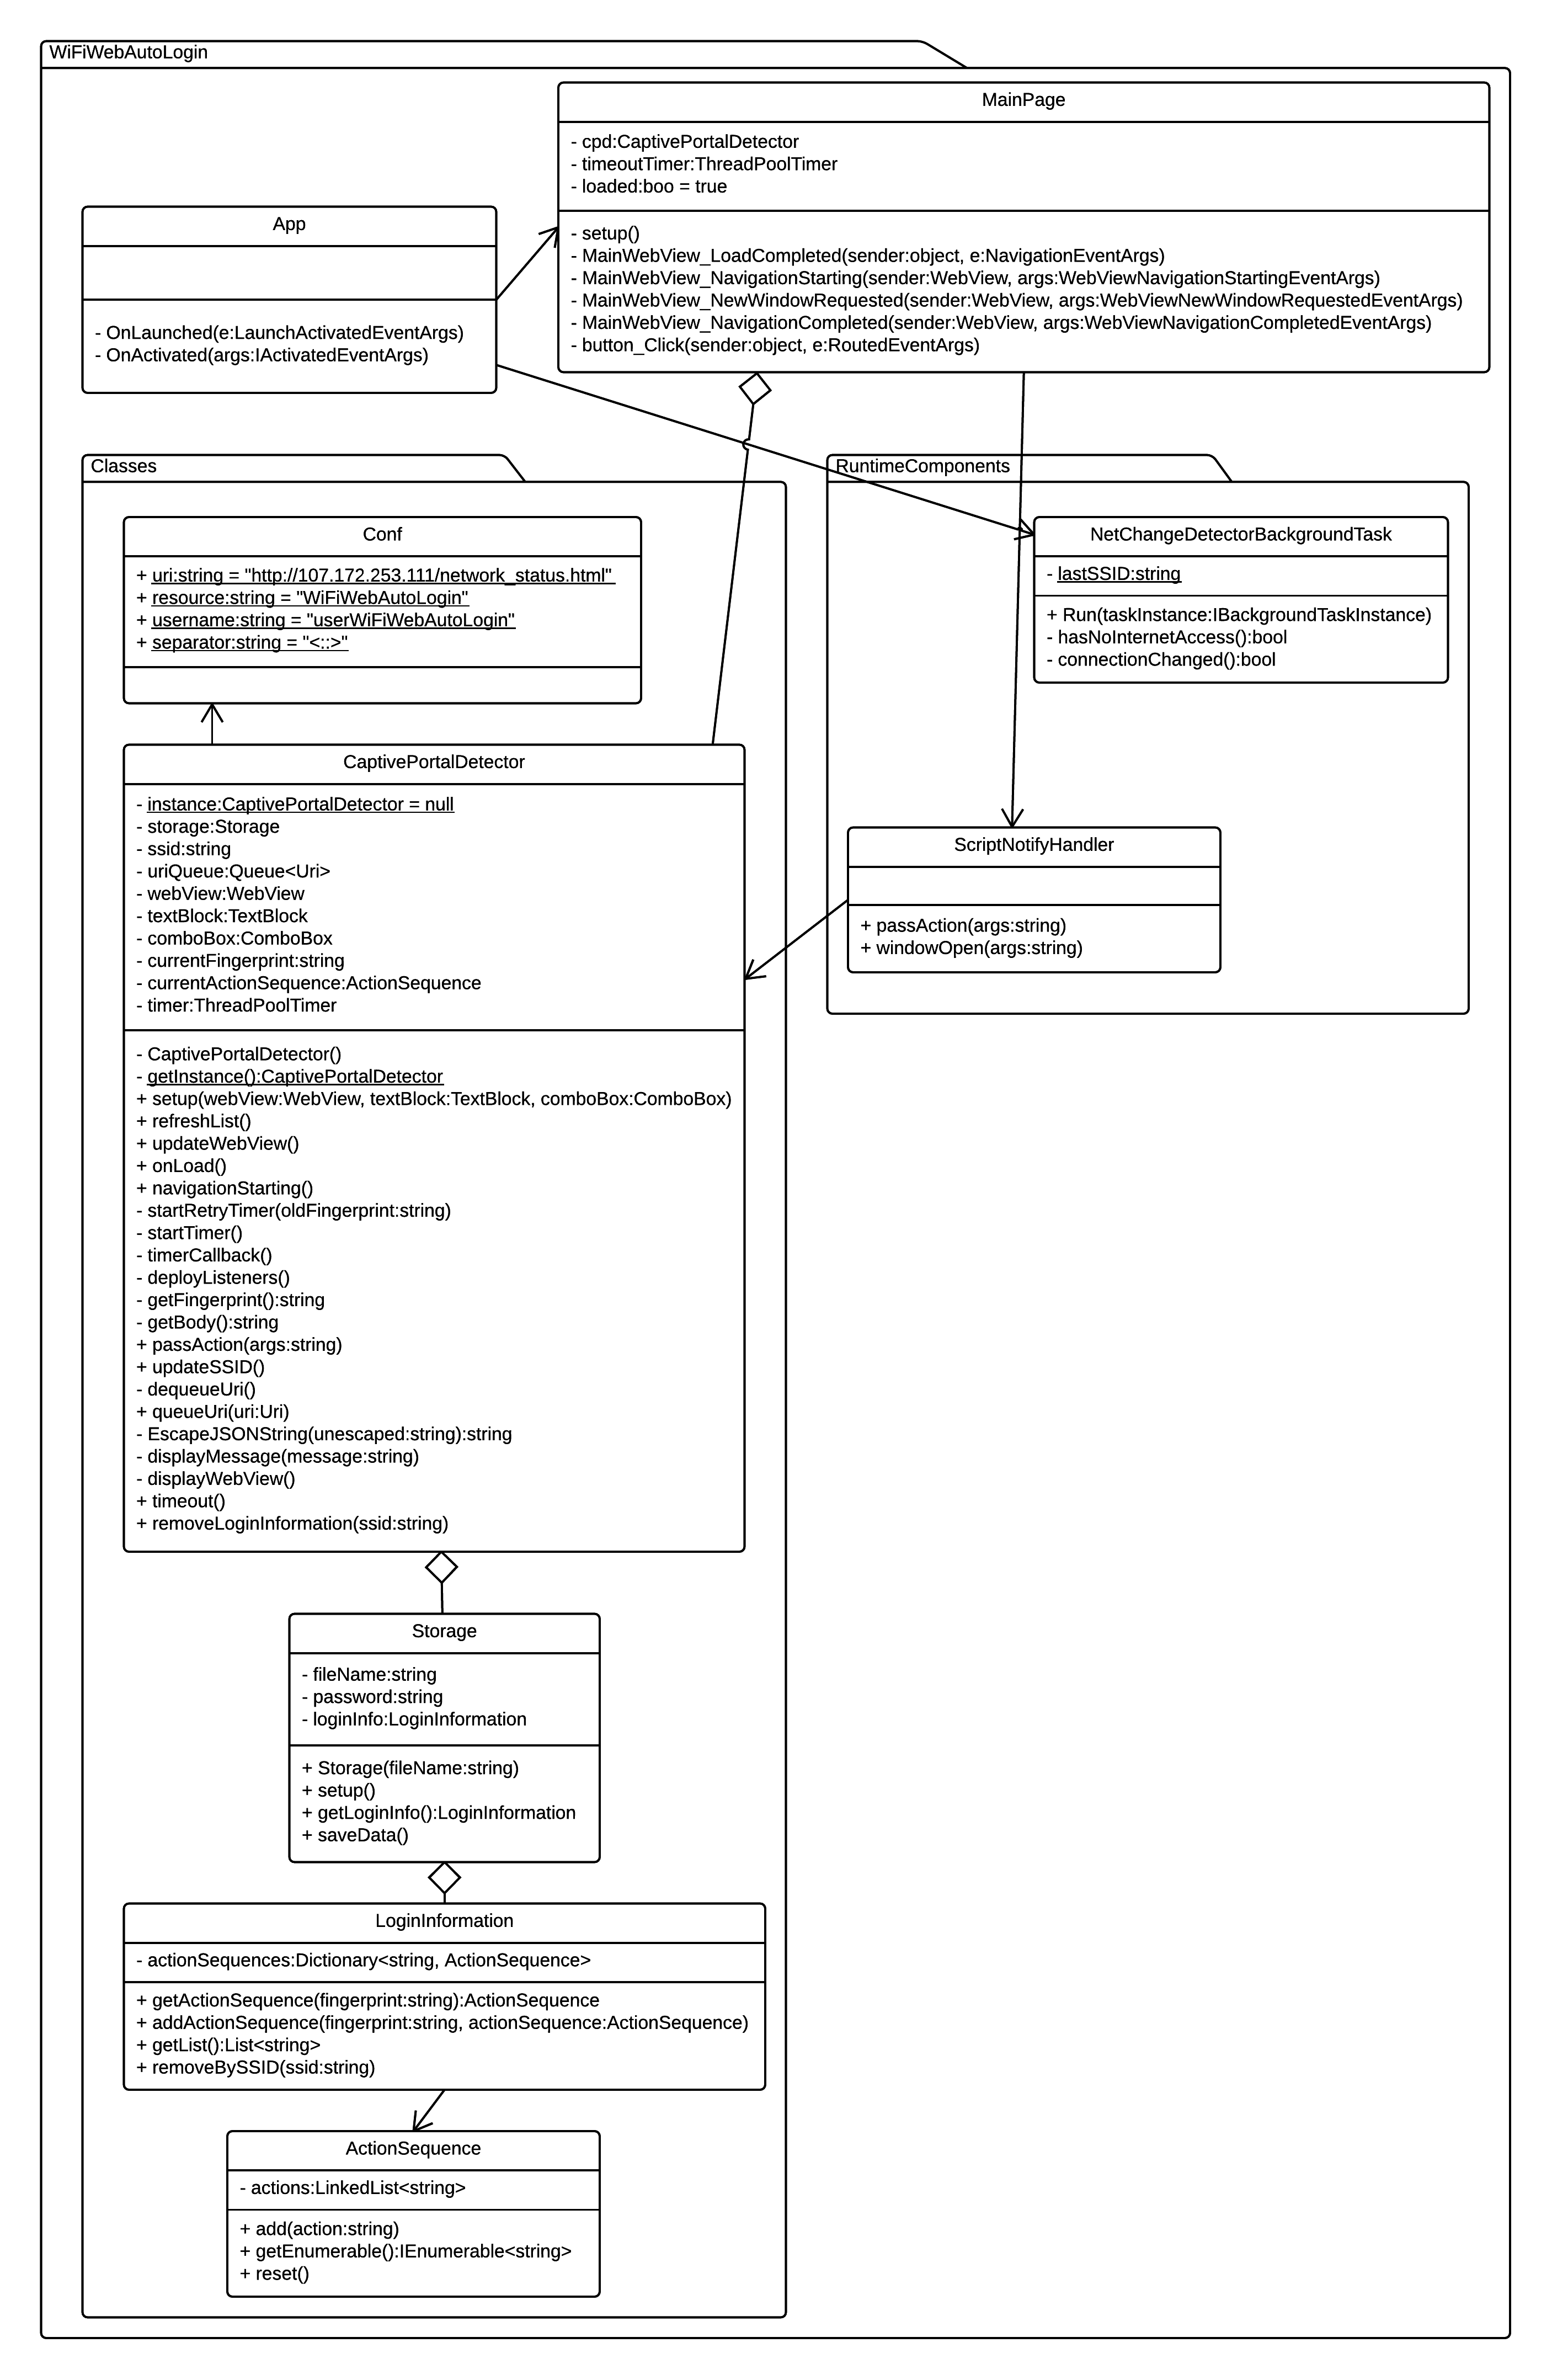
\includegraphics[scale=0.63]{Gambar/DetailedClassDiagram.png}
    \caption[Diagram Kelas Rinci.]{Diagram Kelas Rinci.} 
    \label{fig:DetailedClassDiagram}
\end{figure}

\par{\textbf{CustomBackgroundTask} : Kelas ini merupakan kelas yang digunakan untuk melakukan deteksi perubahan jaringan yang nantinya digunakan untuk menampilkan notifikasi apabila terdeteksi adanya jaringan yang terhubung tanpa adanya internet. Atribut yang dimiliki oleh kelas ini adalah:
    \begin{itemize}
        \item{lastSSID\\Atribut ini menyimpan SSID terakhir yang nantinya akan dibandingkan dengan SSID terbaru untuk mendeteksi adanya perubahan SSID.}
    \end{itemize}
    Metode-metode yang dimiliki oleh kelas ini adalah:
    \begin{itemize}
        \item{Run\\Metode ini dipanggil saat Windows mengalami perubahan jaringan.}
        \item{hasInternetAccess\\Metode ini digunakan untuk medeteksi adanya akses internet menggunakan API yang diberkan oleh UWP.}
        \item{conectionChanged\\Metode ini digunakan untuk medeteksi perubahan SSID.}
    \end{itemize}
}

\par{\textbf{ScriptNotifyHandler} : Kelas ini merupakan kelas yang digunakan untuk menghubungkan sisi javascript pada WebView dengan kode C\#. Metode-metode yang dimiliki oleh kelas ini adalah:
    \begin{itemize}
        \item{passAction\\Metode ini dipanggil saat \textit{listener} yang sudah disisipkan ke dalam WebView mendeteksi \textit{action} yang dapat direkam. \textit{Action} yang direkam berupa teks yang berisi kode javascript yang dapat mereplikasi \textit{action} tersebut.}
        \item{windowOpen\\Metode ini dipanggil saat javascript pada WebView memanggil fungsi window.open atau fungsi open.}
    \end{itemize}
}

\par{\textbf{CaptivePortalDetector} : Kelas ini merupakan kelas utama yang berfungsi untuk melakukan deteksi \textit{captive portal}, menyisipkan kode \textit{listener} pada WebView, merekam \textit{action sequence} yang dilakukan oleh pengguna, dan menjalankan kembali \textit{action sequence} yang sudah tersimpan. Kelas ini menggunakan \textit{design pattern} singleton agar kelas-kelas lainnya bisa mengakses \textit{instance} yang sama pada setiap \textit{session}. Atribut yang dimiliki oleh kelas ini adalah:
    \begin{itemize}
        \item{instance\\Atribut ini menyimpan \textit{instance} CaptivePortalDetector.}
        \item{storage\\Atribut ini menyimpan objek Storage yang digunakan untuk menyimpan dan mengakses informasi login.}
        \item{ssid\\Atribut ini menyimpan SSID saat ini.}
        \item{uriQueue\\Atribut ini menyimpan queue Uri yang perlu diakses.}
        \item{webView\\Atribut ini menyimpan WebView yang digunakan untuk melakukan deteksi \textit{captive portal}.}
        \item{textBlock\\Atribut ini menyimpan TextBlock yang digunakan untuk menampilkan pesan kepada pengguna.}
        \item{comboBox\\Atribut ini menyimpan ComboBox yang digunakan untuk menampilkan daftar SSID yang sudah tersimpan kepada pengguna.}
        \item{currentFingerprint\\Atribut ini menyimpan fingerprint saat ini.}
        \item{currentActionSequence\\Atribut ini menyimpan ActionSequence yang terkait dengan fingerprint saat ini.}
        \item{timer\\Atribut ini menyimpan timer yang digunakan untuk mengatur waktu akses Uri dalam uriQueue.}
    \end{itemize}
    Metode-metode yang dimiliki oleh kelas ini adalah:
    \begin{itemize}
        \item{getInstance\\Metode ini digunakan untuk mendapatkan \textit{instance} dari CaptivePortalDetector.}
        \item{setup\\Metode ini digunakan untuk melakukan \textit{setup} awal yang menyimpan WebView, TextBlock, dan ComboBox ke dalam \textit{instance} CaptivePortalDetector.}
        \item{refreshList\\Metode ini digunakan untuk melakukan \textit{refresh} tampilan ComboBox.}
        \item{updateWebView\\Metode ini digunakan untuk menentukan melakukan deteksi \textit{captive portal} jika terhubung dengan koneksi WiFi, atau menampilkan pesan kepada pengguna juka tidak terhubung dengan koneksi WiFi.}
        \item{onLoad\\Metode ini dipanggil saat WebView sudah selesai melakukan \textit{loading} halaman.}
        \item{onLoad\\Metode ini dipanggil saat WebView sudah selesai melakukan \textit{loading} halaman.}
        \item{navigationStarting\\Metode ini dipanggil saat WebView mulai melakukan navigasi ke halaman baru.}
        \item{passAction\\Metode ini digunakan untuk menyimpan \textit{action} yang dikirimkan oleh ScriptNotifyHandler ke dalam currentActionSequence.}
        \item{updateSSID\\Metode ini digunakan untuk mendapatkan SSID terbaru.}
        \item{queueUri\\Metode ini digunakan untuk memasukkan Uri baru ke dalam uriQueue.}
        \item{timeout\\Metode ini digunakan untuk menyatakan bahwa terjadi \textit{connection timeout}.}
        \item{removeLoginInformation\\Metode ini digunakan untuk menghapus seluruh informasi login yang terkait dengan SSID tertentu.}
    \end{itemize}
}

\par{\textbf{Storage} : Kelas ini digunakan untuk menyimpan informasi login dan password yang digunakan untuk melakukan enkripsi. Atribut yang dimiliki oleh kelas ini adalah:
    \begin{itemize}
        \item{fileName\\Atribut ini menyimpan nama file yang digunakan untuk menyimpan informasi login yang terenkripsi.}
        \item{password\\Atribut ini menyimpan password yang digunakan untuk melakukan enkripsi.}
        \item{loginInfo\\Atribut ini menyimpan objek LoginInformation yang digunakan untuk menyimpan seluruh informasi login.}
    \end{itemize}
    Metode-metode yang dimiliki oleh kelas ini adalah:
    \begin{itemize}
        \item{setup\\Metode ini digunakan untuk melakukan \textit{setup} awal seperti membuka file dan melakukan dekripsi.}
        \item{getLoginInfo\\Metode ini digunakan untuk mendapatkan objek LoginInformation.}
        \item{saveData\\Metode ini digunakan untuk menyimpan data yang ada pada objek LoginInformation ke dalam file dan melakukan enkripsi pada file tersebut.}
    \end{itemize}
}

\par{\textbf{LoginInformation} : Kelas ini digunakan untuk merepresentasikan informasi login. Atribut yang dimiliki oleh kelas ini adalah:
    \begin{itemize}
        \item{actionSequences\\Atribut ini merupakan pasangan \textit{key-value} antara suatu fingerprint dengan ActionSequence.}
    \end{itemize}
    Metode-metode yang dimiliki oleh kelas ini adalah:
    \begin{itemize}
        \item{getActionSequence\\Metode ini digunakan untuk mendapatkan ActionSequence berdasarkan fingerprint tertentu.}
        \item{addActionSequence\\Metode ini digunakan untuk menambahkan ActionSequence untuk fingerprint tertentu.}
        \item{removeBySSID\\Metode ini digunakan untuk menghapus ActionSequence milik fingerprint tertentu.}
        \item{getList\\Metode ini digunakan untuk mendapatkan daftar SSID yang sudah direkam.}
    \end{itemize}
}

\par{\textbf{ActionSequence} : Kelas ini digunakan untuk merepresentasikan urutan \textit{action}. Atribut yang dimiliki oleh kelas ini adalah:
    \begin{itemize}
        \item{actions\\Atribut ini merupakan daftar \textit{action} yang berupa kode javascript.}
    \end{itemize}
    Metode-metode yang dimiliki oleh kelas ini adalah:
    \begin{itemize}
        \item{add\\Metode ini digunakan untuk menambahkan \textit{action} ke dalam daftar ini.}
        \item{getEnumerable\\Metode ini digunakan untuk mendapatkan enumerable dari daftar \textit{actions}, sehingga mempermudah eksekusi \textit{actions}.}
        \item{reset\\Metode ini digunakan untuk menghapus seluruh \textit{action} yang ada pada daftar ini.}
    \end{itemize}
}



\section{Perancangan Interaksi Perangkat Lunak}
\label{sec:perancangan_interaksi}

\subsection{Perancangan Interaksi Deteksi Jaringan}
\label{subsec:perancangan_interaksi_deteksi_jaringan}

\begin{figure}[!htb]
    \centering
    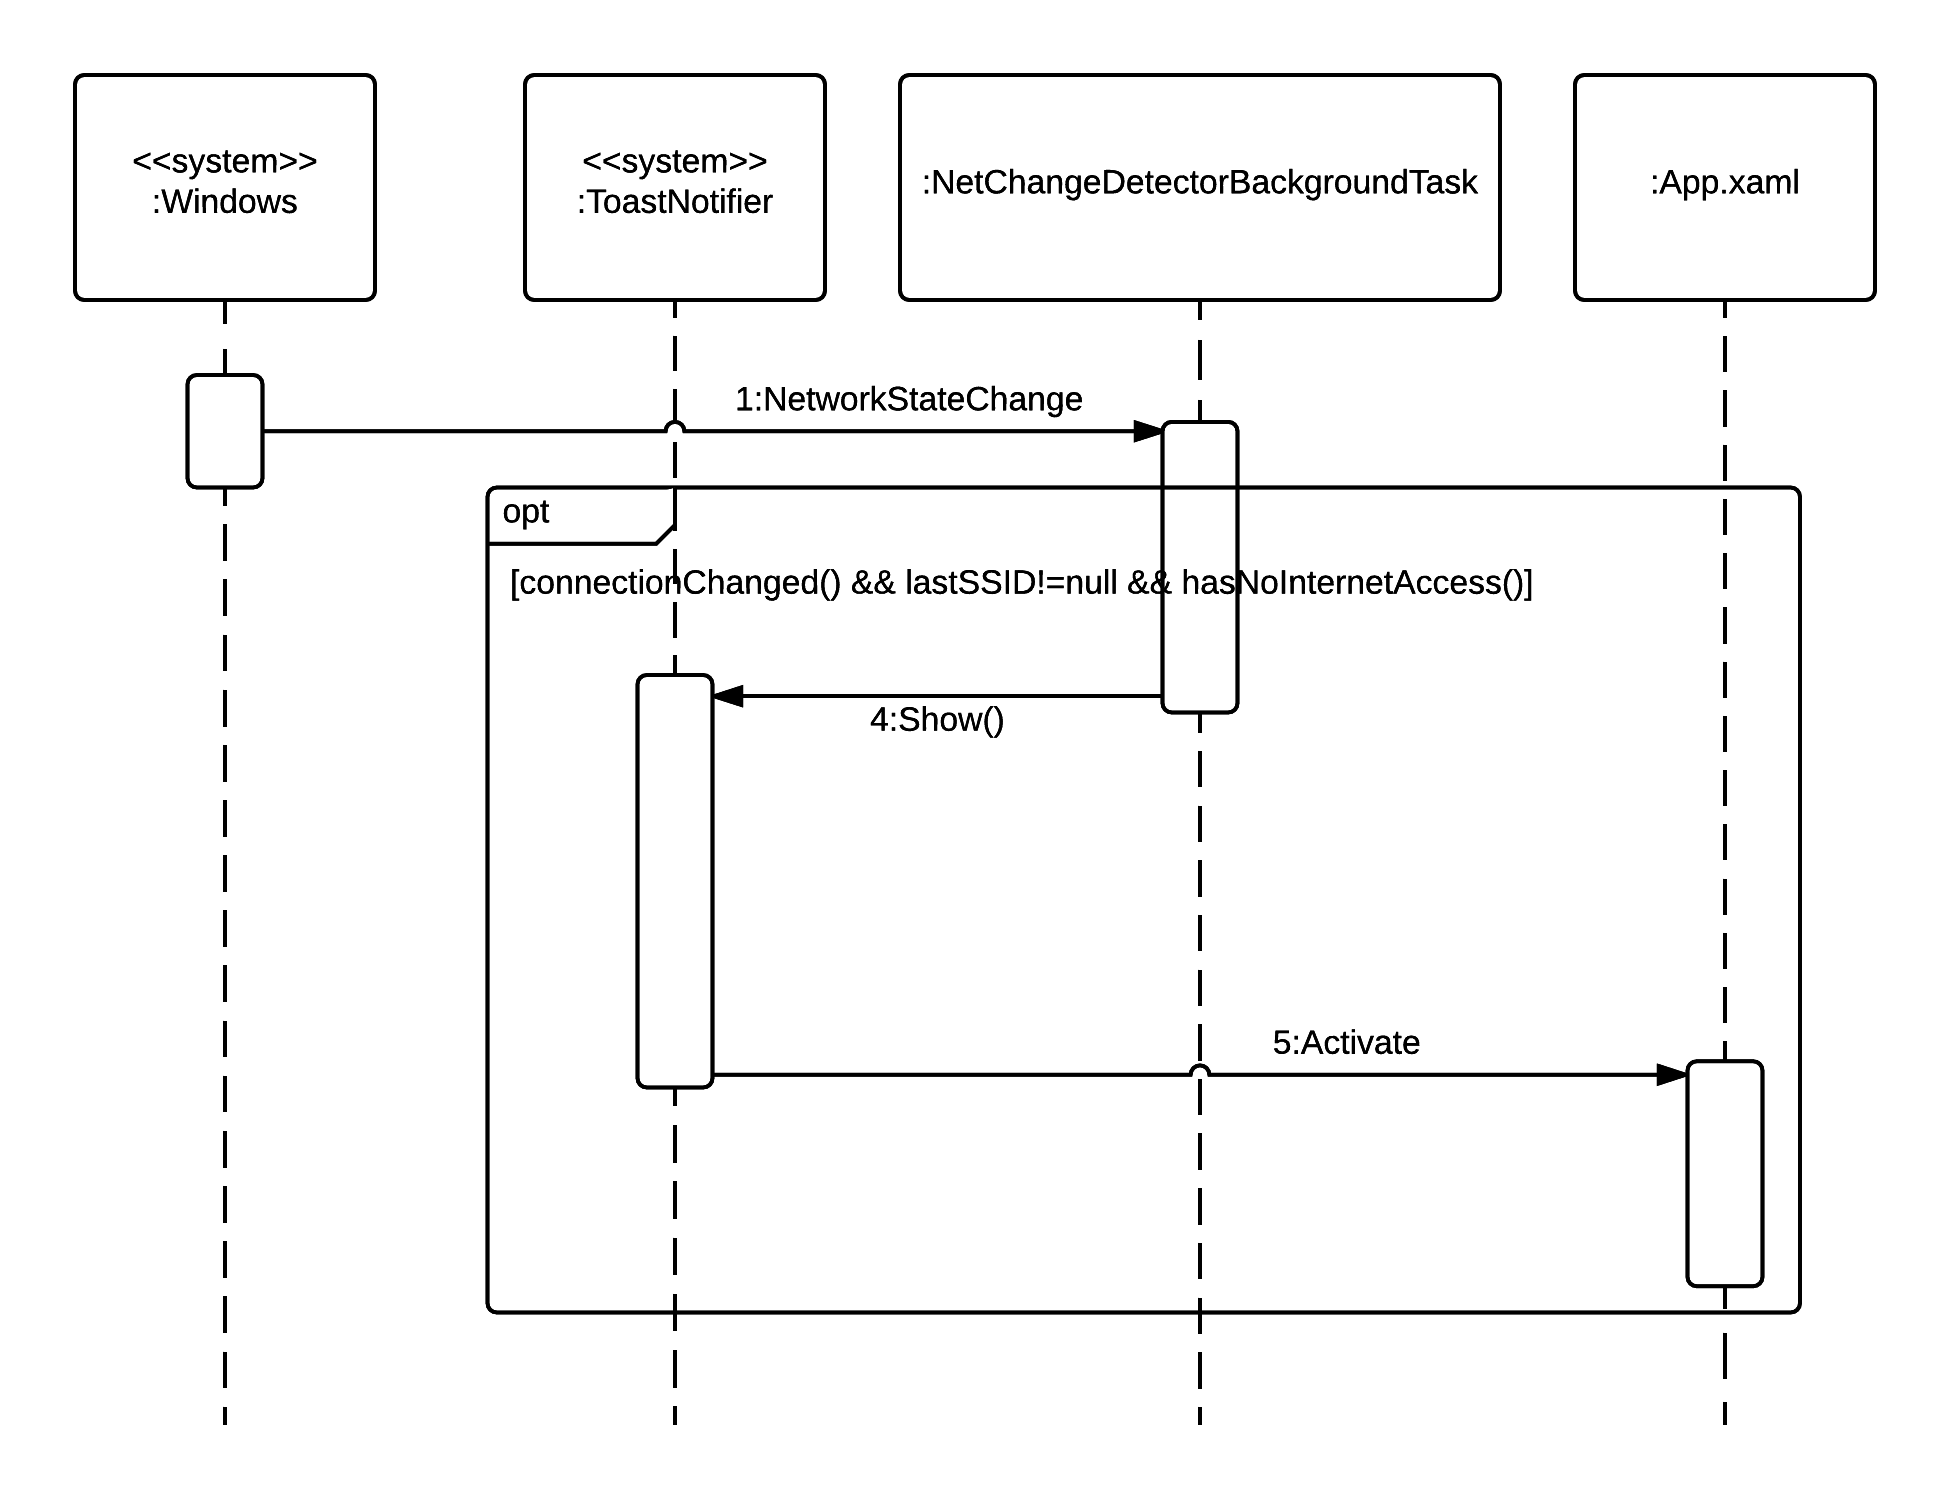
\includegraphics[scale=0.9]{Gambar/SequenceDiagramNetworkDetection.png}
    \caption[Diagram Interaksi Deteksi Jaringan.]{Diagram Interaksi Deteksi Jaringan.} 
    \label{fig:NetworkDetectionSequenceDiagram}
\end{figure}

Gambar \ref{fig:NetworkDetectionSequenceDiagram} menjelaskan mengenai interaksi antar objek dalam perangkat lunak untuk melakukan deteksi perubahan jaringan.

\subsection{Perancangan Interaksi Penciptaan Password}
\label{subsec:perancangan_interaksi_penciptaan_password}

\begin{figure}[!htb]
    \centering
    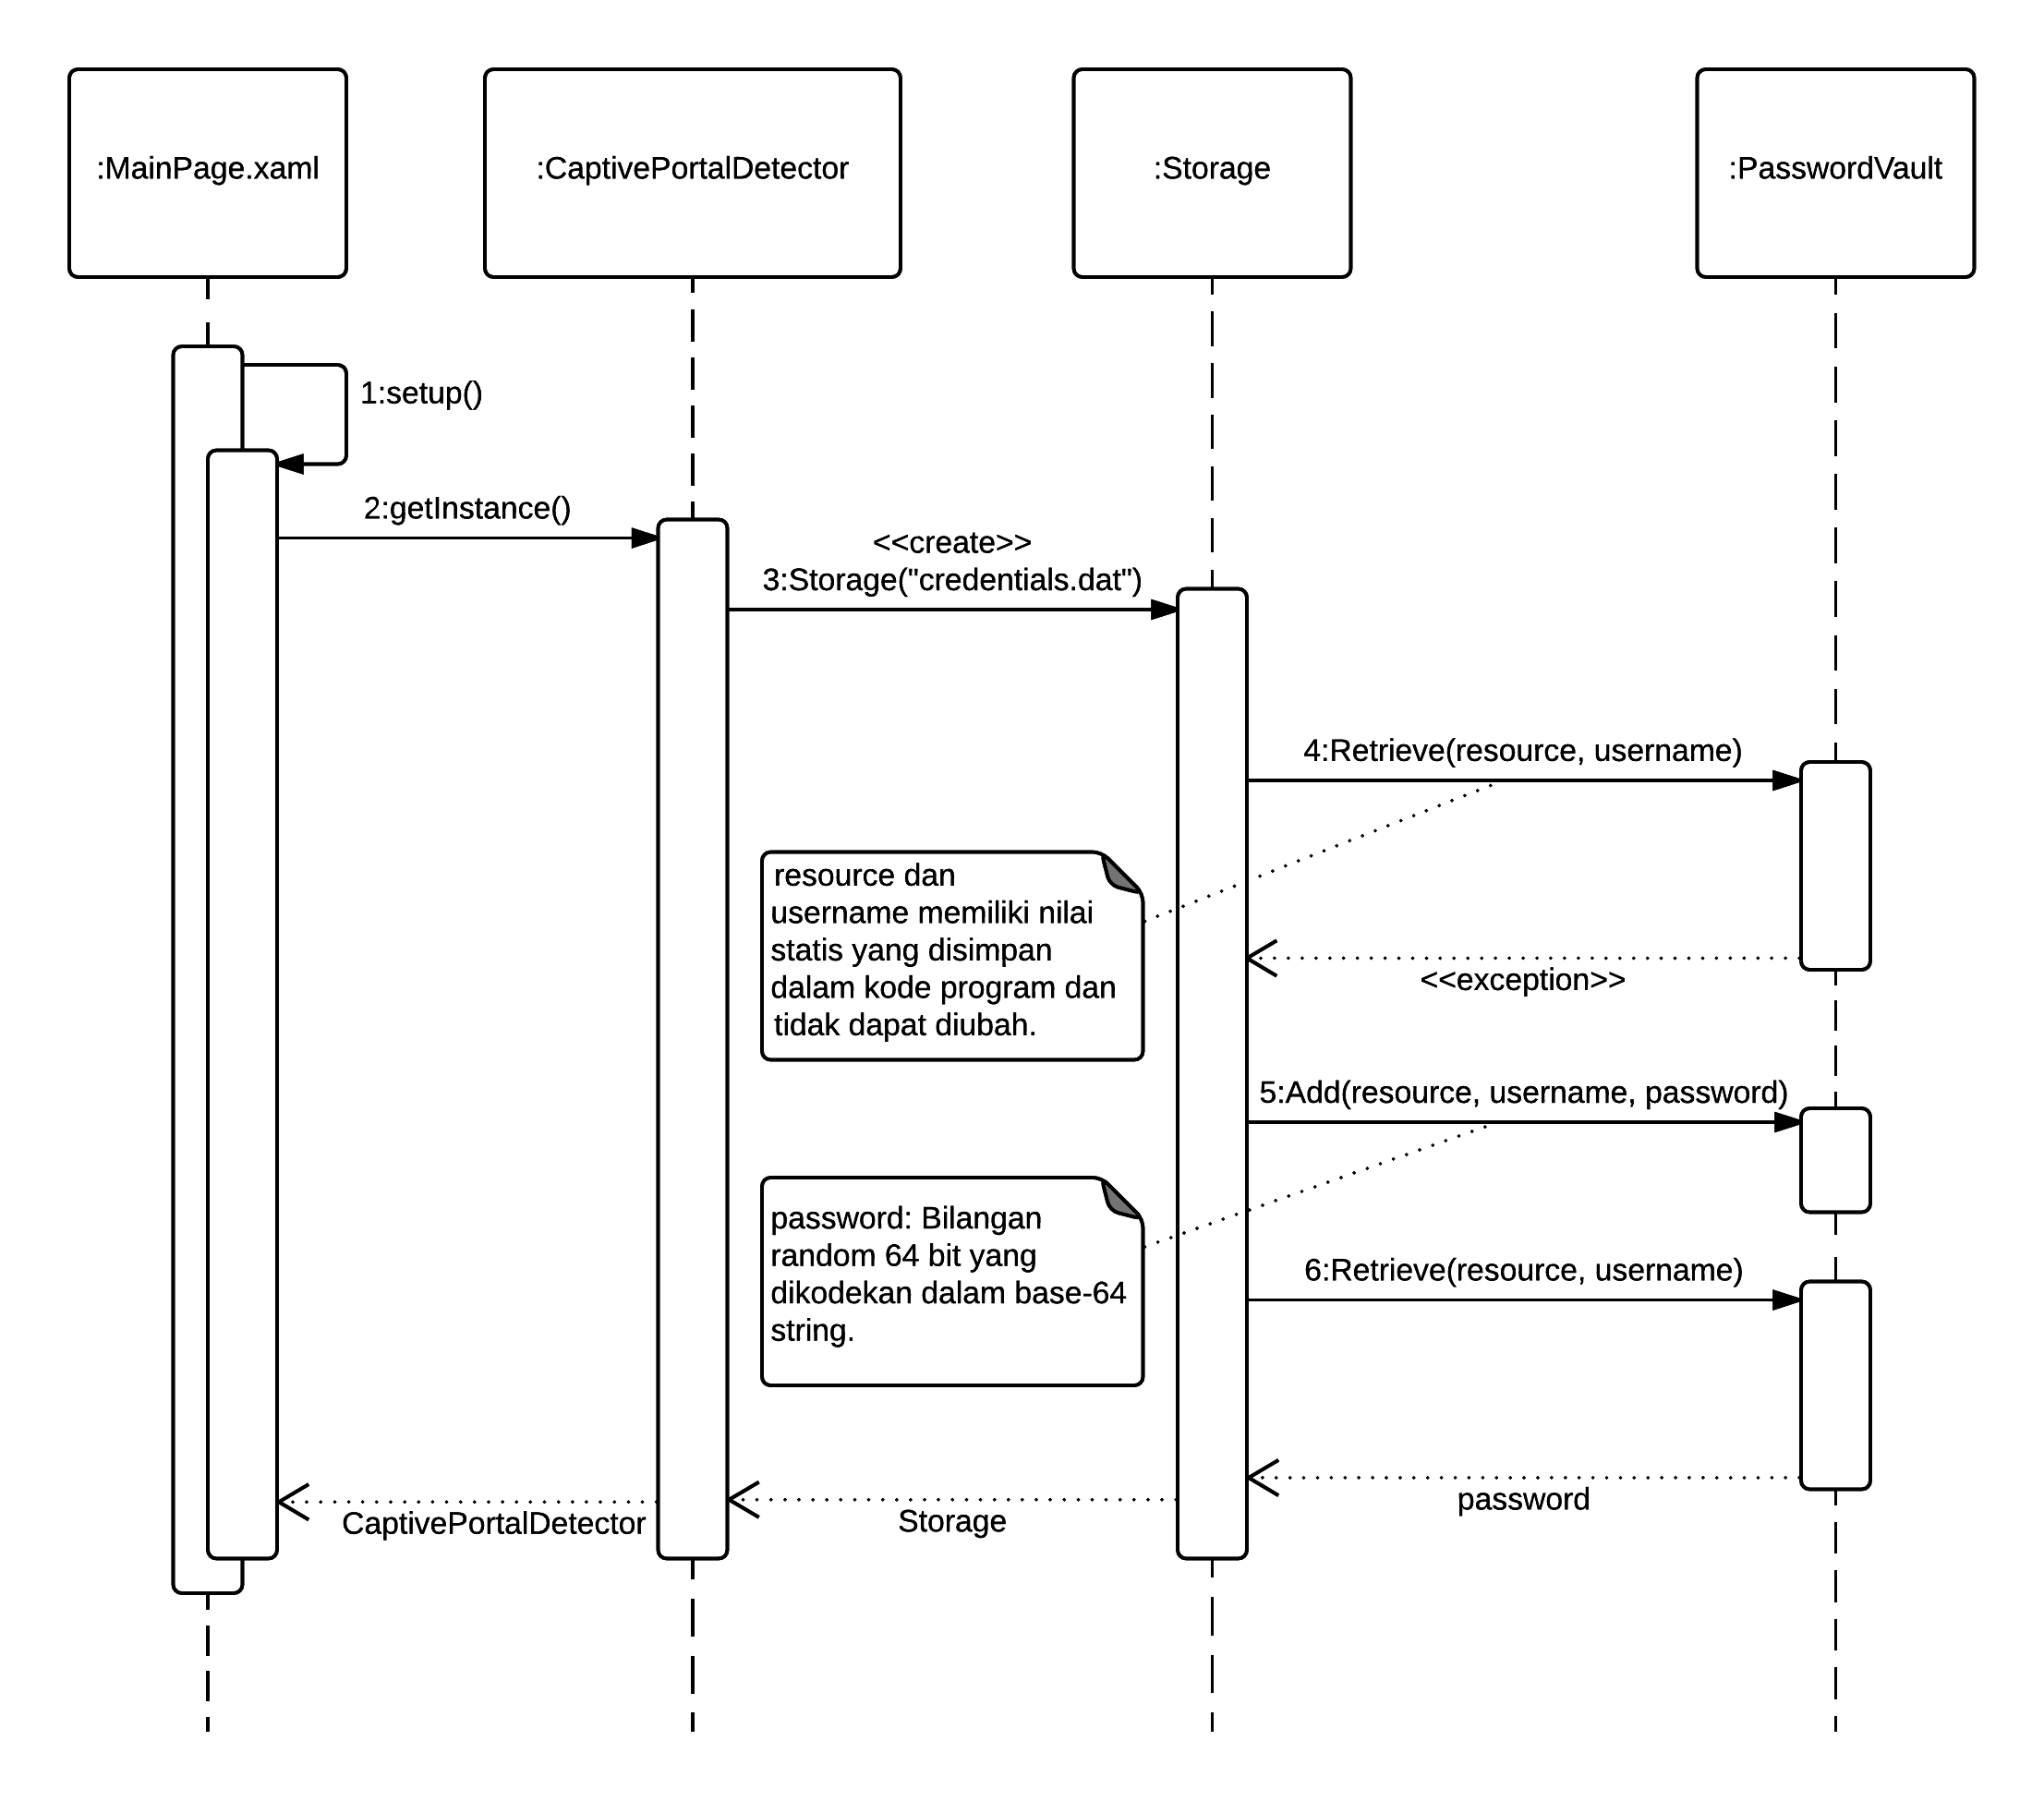
\includegraphics[scale=0.9]{Gambar/SequenceDiagramPasswordGeneration.png}
    \caption[Diagram Interaksi Penciptaan Password.]{Diagram Interaksi Penciptaan Password.} 
    \label{fig:PasswordGenerationSequenceDiagram}
\end{figure}

Gambar \ref{fig:PasswordGenerationSequenceDiagram} menjelaskan mengenai interaksi antar objek dalam perangkat lunak untuk menciptakan password random saat perangkat lunak pertama kali dijalankan.

\subsection{Perancangan Interaksi Penyimpanan Informasi Login}
\label{subsec:perancangan_interaksi_penciptaan_password}

\begin{figure}[!htb]
    \centering
    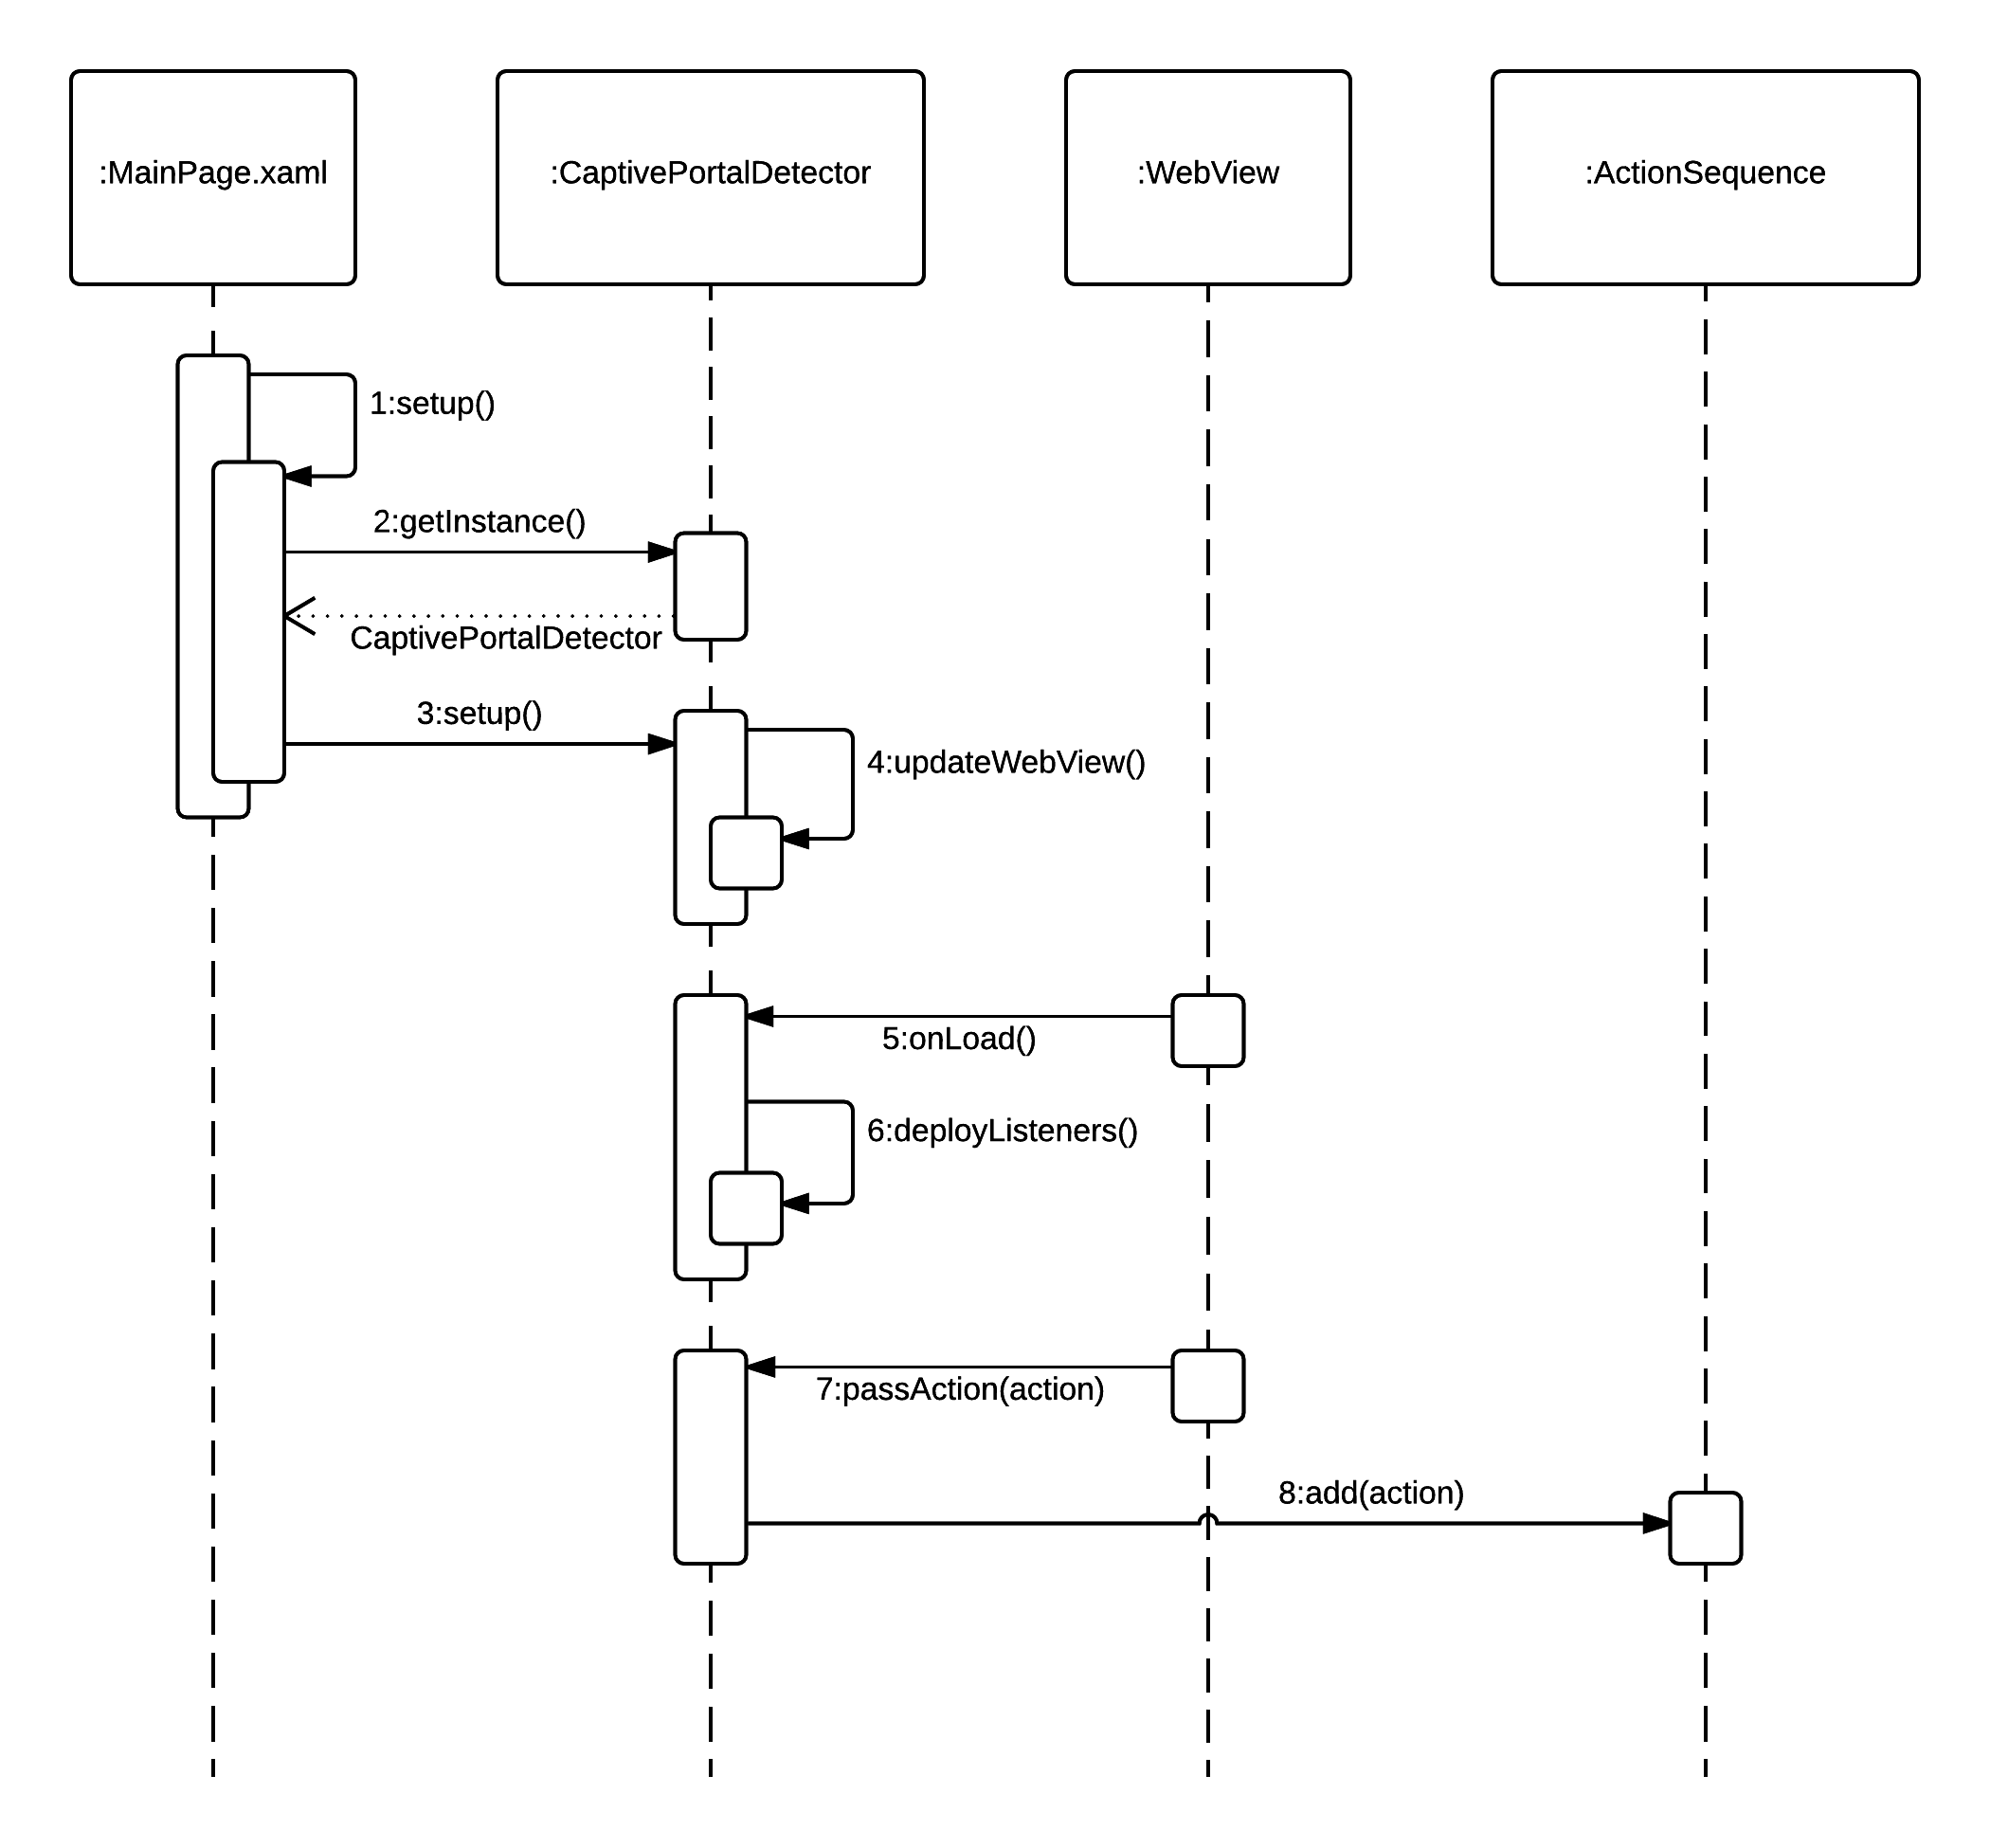
\includegraphics[scale=0.9]{Gambar/SequenceDiagramLoginInformationSaving.png}
    \caption[Diagram Interaksi Penyimpanan Informasi Login.]{Diagram Interaksi Penyimpanan Informasi Login.} 
    \label{fig:LoginInformationSavingSequenceDiagram}
\end{figure}

Gambar \ref{fig:LoginInformationSavingSequenceDiagram} menjelaskan mengenai interaksi antar objek dalam perangkat lunak untuk menyimpan informasi login.
